% !TEX root = ../paper.tex
\documentclass[../paper.tex]{subfiles}
\begin{document}
Разаботанная аппаратная часть должна отвечать следующим условиям. Прием сигнала стетоскопом осуществляется через микрофон. Далее, сигнал с микрофона должен подаваться на усилитель, усиливающий сигнал с микрофона до значений, в которых работает аналого цифровой преобразователь. Аналого цифровой преобразователь принимает сигнал и подключается к компьютеру через USB порт для передачи данных. Врач должен иметь возможность прослушивать пациента, видеть визуализацию сигнала на компьютере. Также врач должен иметь возможность увидеть спектр сигнала после преобразования Фурье. Преобразование Фурье должно производиться как на локальном компьютере, так и на удаленном сервере.

Разработанная информационная система состоит из следующих частей:
\begin{enumerate}
  \item Врач
  \item Пациент (диагностируемый)
  \item Микрофон
  \item Усилитель
  \item Аналого цифровой преобразователь
  \item Компьютер
  \item Удаленный сервер для высокопроизводительных вычислений
\end{enumerate}

\begin{figure}[H]
\centering
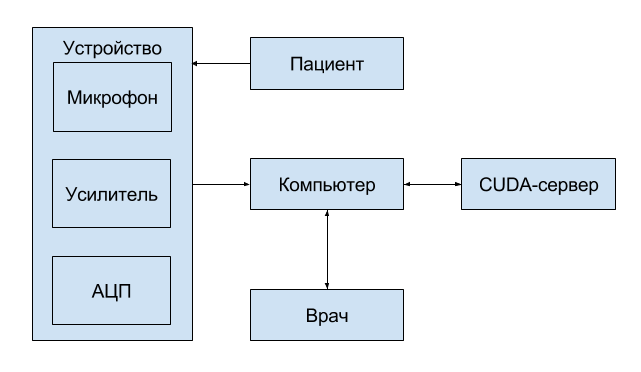
\includegraphics[width=\textwidth]{images/blueprint.png}
\caption{Схема програмно-аппаратной системы}
\end{figure}

\begin{figure}[H]
\centering
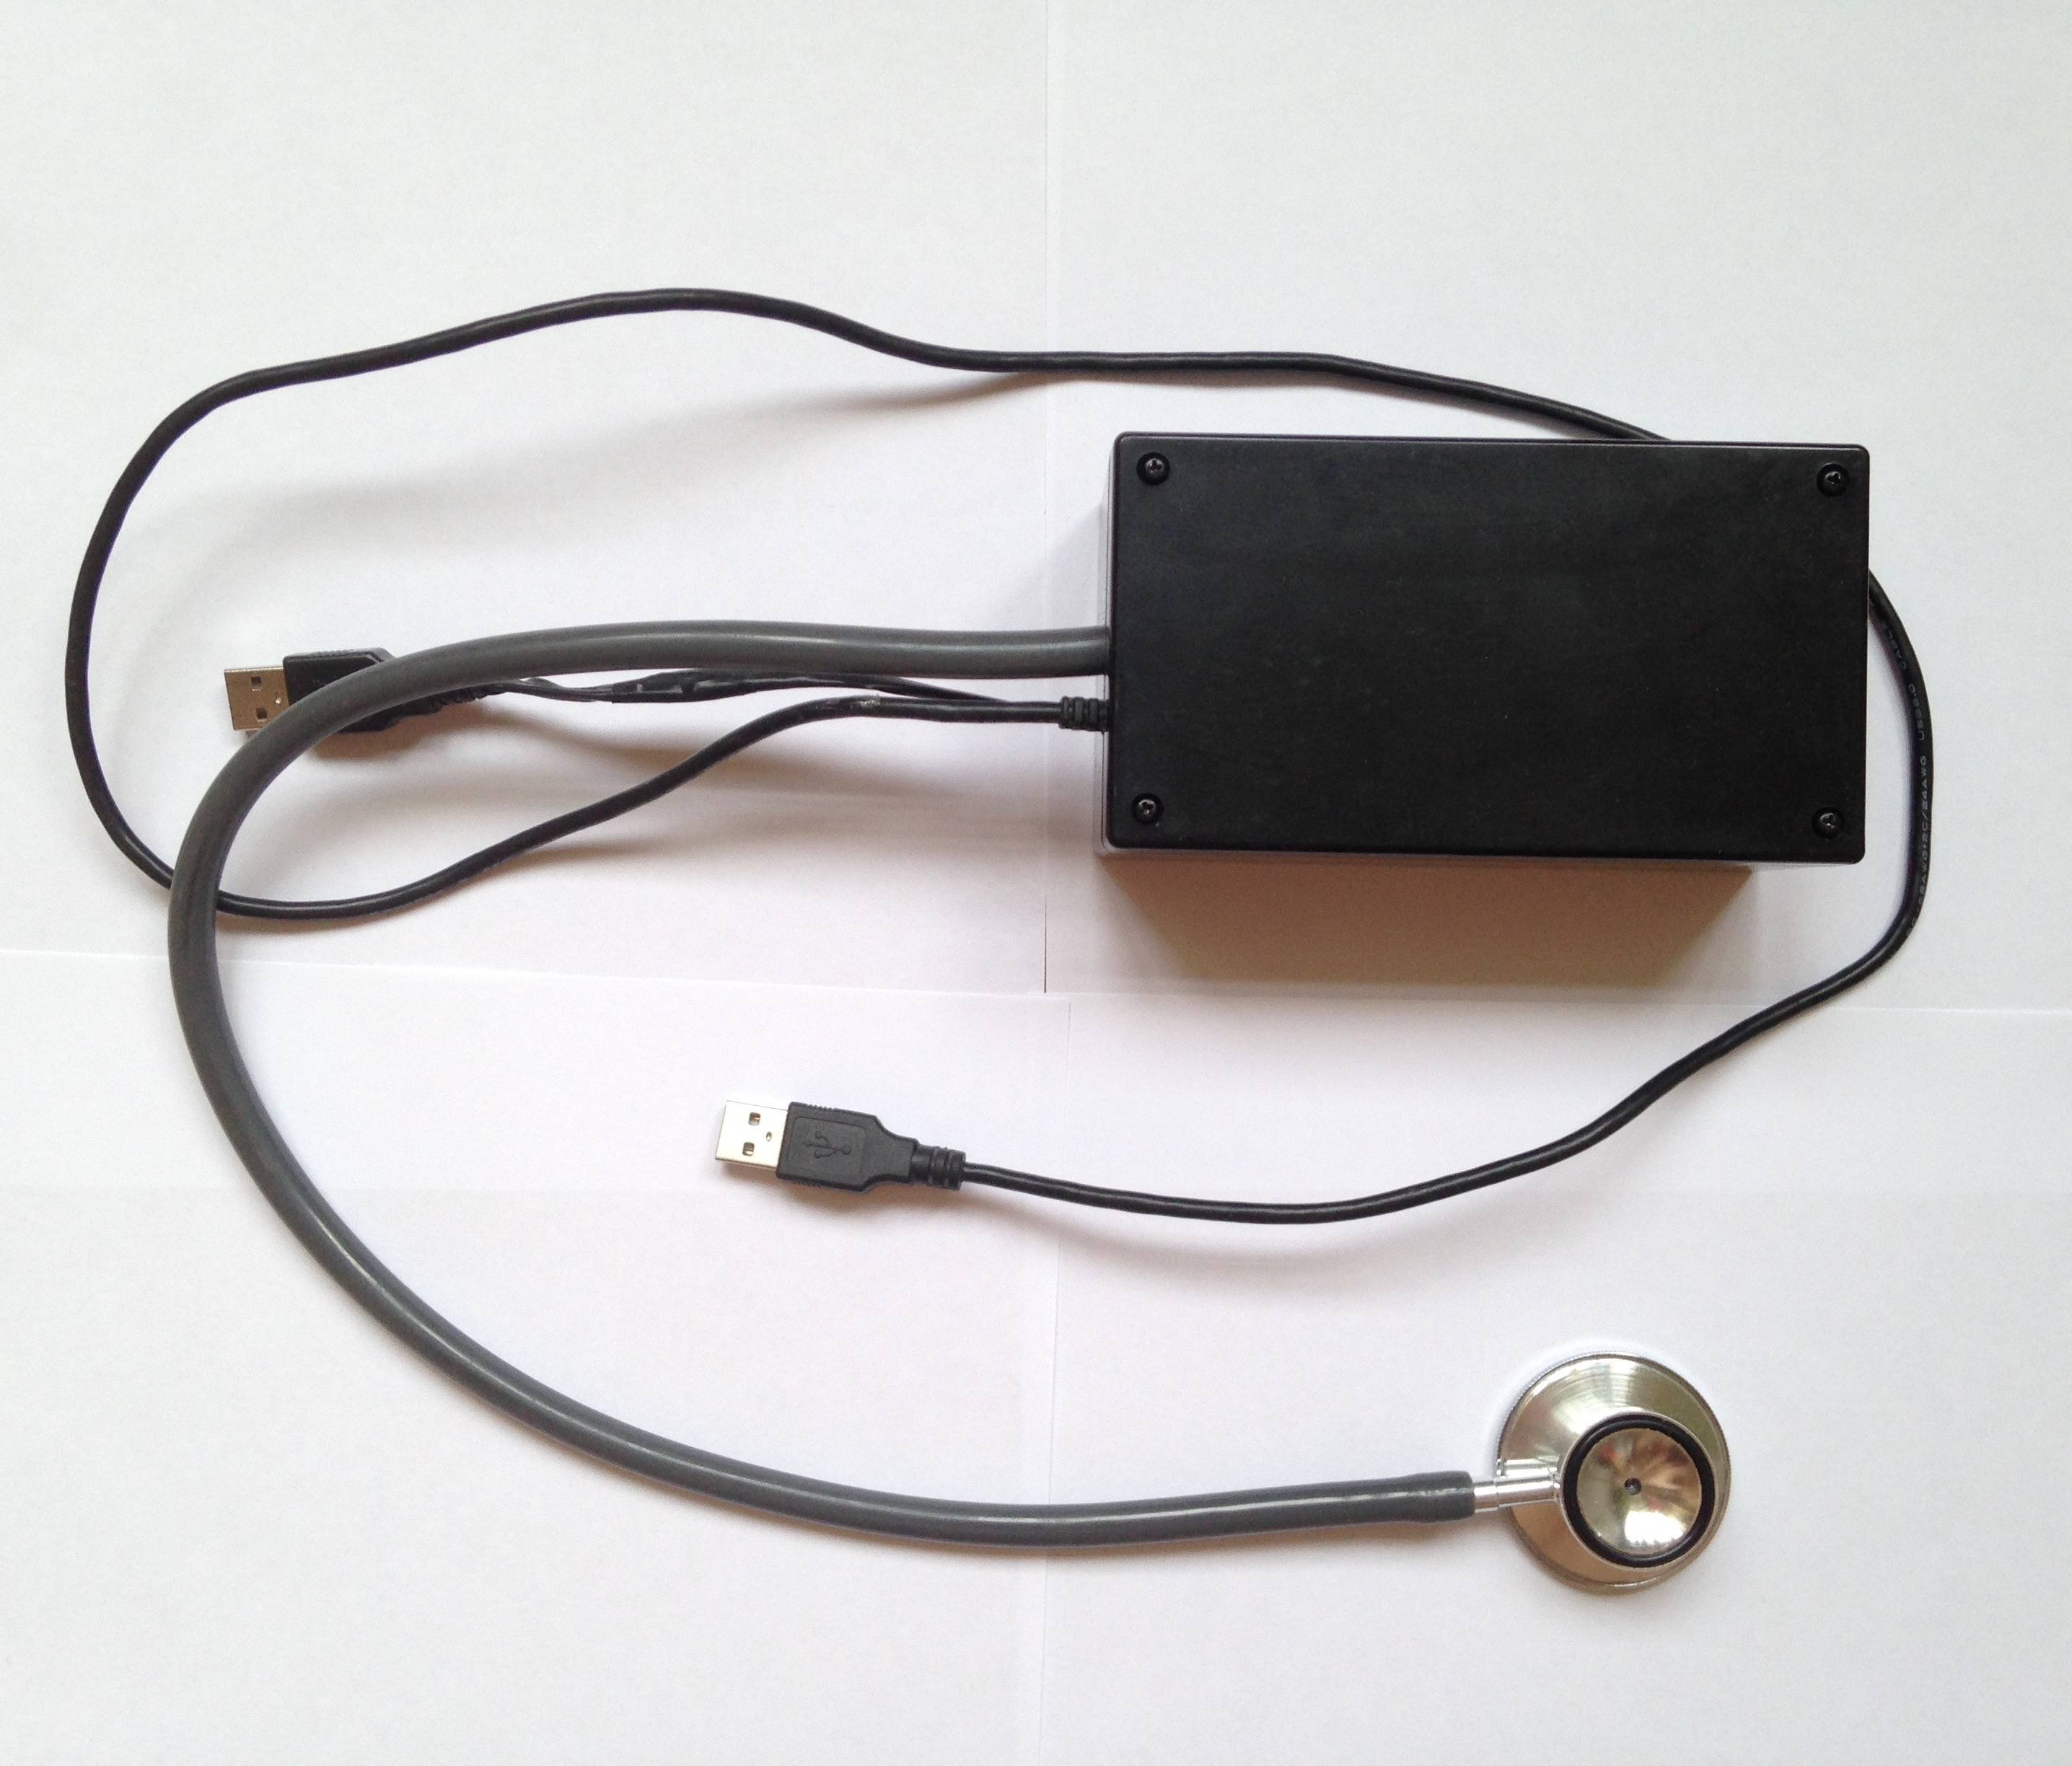
\includegraphics[width=15cm]{images/hardware.jpg}
\caption{Собранный прототип}
\end{figure}

\subsection{Описание микрофона}
В качестве микрофона был выбран SWEN MK-200. Микрофон был вынут из стандартного корпуса, чтобы лучше соединиться с трубкой, ведущей к мембране. \\

\begin{table}[h]
\centering
\caption{Технические характеристики SWEN MK-200}
\begin{tabular}{|l|l|}
\hline
Чувствительность, дБ           & -60 ± 3                    \\ \hline
Диапазон частот, Гц            & 50 – 16 000                \\ \hline
Размер микрофонного модуля, мм & 9×7                        \\ \hline
Тип разъема                    & мини-джек Ø 3,5 мм (3 pin) \\ \hline
Длина кабеля, м                & 1,8                        \\ \hline
Вес, г                         & 63                         \\ \hline
\end{tabular}
\end{table}

Наилучшая чувствительность данного микрофона достигается в диапазоне частот от 50 до 16000 Гц. Тем не менее, микрофон с ослаблением принимает сигнал вплоть до 40кГц. Поэтому данный микрофон подходит для данного проекта.

Для подавления шумов и лучшей передачи звука от сердца, легких и других органов к микрофону присоединяются мембрана и соединительная трубка от аналогового стетоскопа.

\subsection{Описание усилителя}
Усилитель для микрофона был создан самостоятельно в рамках данной работы.

Была выбрана следующая схема усилителя:

\begin{figure}[H]
\centering
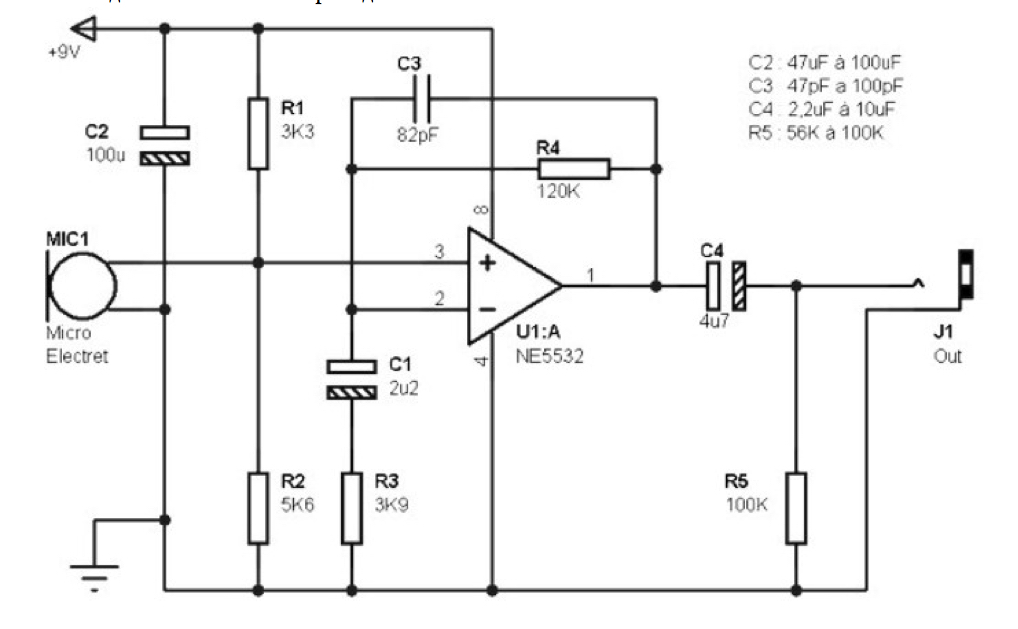
\includegraphics[width=14cm]{images/circuit.jpg}
\caption{Схема усилителя сигнала}
\end{figure}

В качестве операционного усилителя был выбран \textbf{MCP6022} от производителя Microchip. Это усилитель типа Rail-to-Rail SO-8.

SOIC или просто SO (small-outline-integrated-circuit), а также SOP (Small-Outline Package) корпус микросхем, предназначенный для поверхностного монтажа, занимающий на печатной плате на 30-50\% меньше площади чем аналогичный корпус DIP, а также имеющий на 50-70\% меньшую толщину. Обычно в обозначении также указывается число выводов.

Ниже приводятся параметры операционного усилителя.

\begin{table}[h]
\centering
\caption{Технические характеристики операционного усилителя MCP6022}
\begin{tabular}{|l|l|}
\hline
Полоса частот                  & 10МГц                      \\ \hline
Уровень шума                   & 8.7 нВ/√Гц                 \\ \hline
Количество каналов             & 2                          \\ \hline
Напряжение питания             & 2.5В --- 5.5В              \\ \hline
Напряжение смещения            & $\pm500\mu V $             \\ \hline
Гармонические искажения        & 0.00053\%                  \\ \hline
Температурный диапазон         & -40°C --- +85°C            \\ \hline
Тип корпуса                    & SO-8                       \\ \hline
\end{tabular}
\end{table}

\begin{figure}[H]
\centering
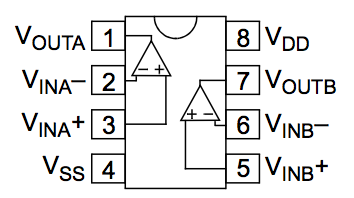
\includegraphics[width=16cm]{images/op-amp.png}
\caption{Распиновка операционного усилителя}
\end{figure}

В данный усилитель встроены High-Pass и Low-Pass фильтры. High-Pass фильтрует частоты сигнала меньше 1Гц. Low-Pass фильтрует частоты выше 100кГц. Меняя конденсатор С3, можно менять частоту среза LowPass фильтра. Усиление схемы зависит от резисторов R3 и R4. На текущий момент усиление составляет порядка 100.

\begin{figure}[H]
\begin{subfigure}{0.5\textwidth}
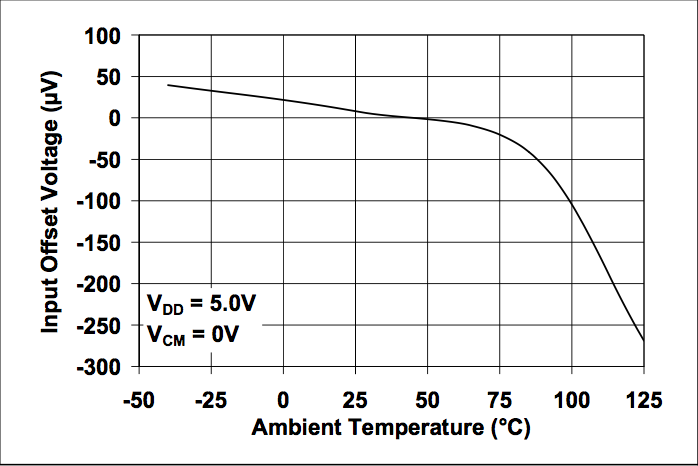
\includegraphics[width=0.9\linewidth, height=5cm]{images/op-amp-plot1.png} 
\caption{Напряжение смещения --- Температура}
\end{subfigure}
\begin{subfigure}{0.5\textwidth}
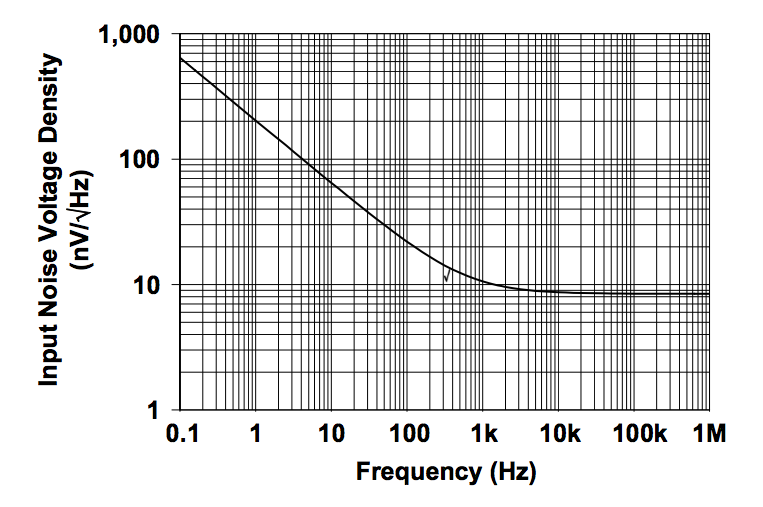
\includegraphics[width=0.9\linewidth, height=5cm]{images/op-amp-plot2.png}
\caption{Шум --- Частота}
\end{subfigure}
\end{figure}

\begin{figure}[H]

\vspace{10mm} % vertical space
 
\begin{subfigure}{0.5\textwidth}
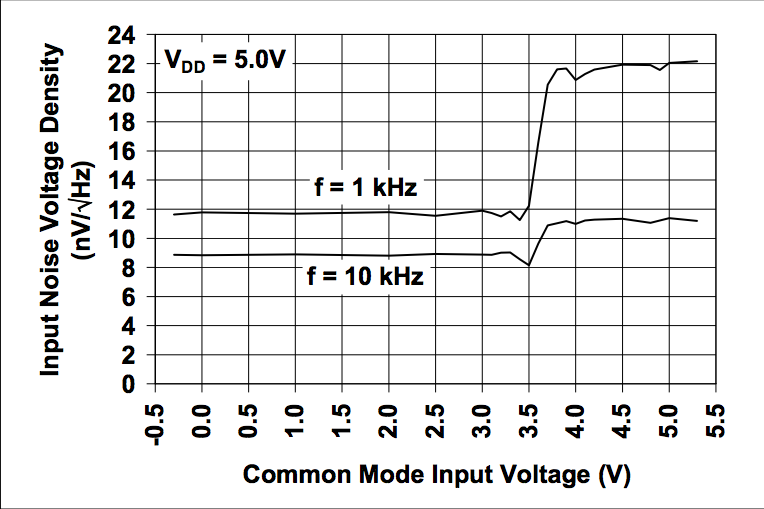
\includegraphics[width=0.9\linewidth, height=5cm]{images/op-amp-plot3.png} 
\caption{Шум - Напряжение смещения}
\end{subfigure}
\begin{subfigure}{0.5\textwidth}
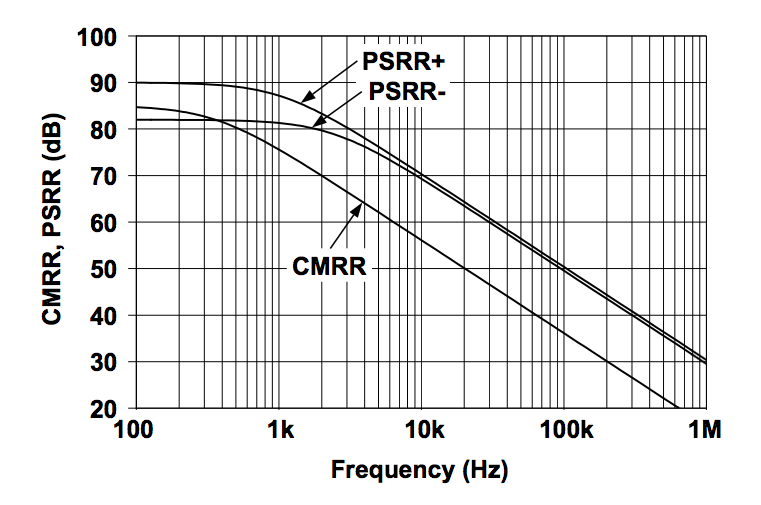
\includegraphics[width=0.9\linewidth, height=5cm]{images/op-amp-plot4.png}
\caption{CMRR --- Частота}
\end{subfigure}

\vspace{10mm} %vertical space

\begin{subfigure}{0.5\textwidth}
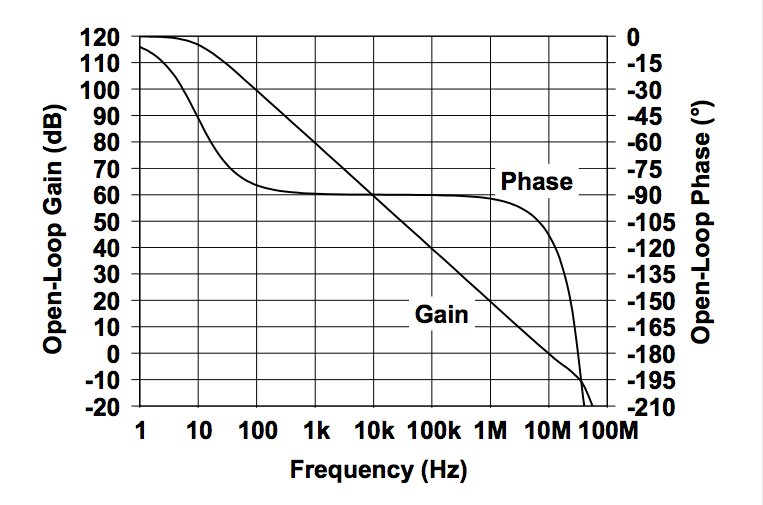
\includegraphics[width=0.9\linewidth, height=5cm]{images/op-amp-plot5.png} 
\caption{Коэффициент усиления - Частота}
\end{subfigure}
\begin{subfigure}{0.5\textwidth}
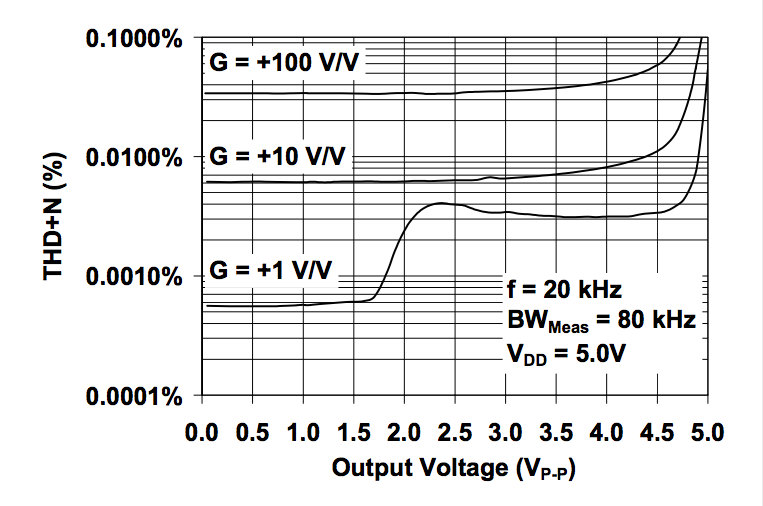
\includegraphics[width=0.9\linewidth, height=5cm]{images/op-amp-plot6.png}
\caption{\small{Гармонические искажения --- Вых. напряжение (f=20кГц)}}
\end{subfigure}

\caption{Параметры операционного усилителя}
\end{figure}

Разработка платы усилителя велась в программе Sprint Layout. Ниже представлен скриншот макета платы из этой программы.

\begin{figure}[H]
\centering
% \includegraphics[width=14cm]{sprint-layout-circuit.png}
\includegraphics[width=10cm]{images/sprint-layout-circuit.png}
\caption{Схема печатной платы усилителя}
\end{figure}

Печатная плата изготавливалась при помощи печати на лазерном принтере методом травления текстолита. 

\subsection{АЦП}
Предназначение АЦП – преобразование непрерывных (аналоговых) входных сигналов в цифровую форму для дальнейшей обработки с помощью компьютера.

В качестве аналого цифрового преобразователя были опробованы 3 устройства:
\begin{enumerate}
  \item LCard E14-140M
  \item ЗАО "Руднев-Шиляев" ЛА-н10-12USB
  \item Arduino Due
\end{enumerate}

\subsubsection{LCard E14-140M}

\begin{table}[H]
\centering
\caption{Технические характеристики АЦП LCard E14-140M}
\begin{tabular}{|l|l|}
                                                                                     \hline
Количество каналов                 & 16 дифференциальных или 32 \\& с "общей землей" \\ \hline
Максимальная частота дискретизации & 200 кГц                                         \\ \hline
Объем буффера памяти               & 64 Кбайт                                        \\ \hline
Разрядность                        & 14 (бит)                                        \\ \hline
Эффективная разрядность            & 13.3 бит (при частоте дискр. 100 кГц)            \\ \hline
Входное сопротивление              & не меньше 10 МОм                                 \\ \hline
Диапазоны входного напряжения      & $\pm10V;\pm2.5V;\pm0.6V;\pm0.15V$               \\ \hline
Синхронизация                      & От внешнего синхро-сигнала, \\& по уровню аналогового, \\& внутренняя. Возможна многомодульная.          \\ \hline
Защита входов                      & 30V (при вкл. питании); 10В (при выкл. \\&питании \\& и в suspend-mode)       \\ \hline
\end{tabular}
\end{table}

\begin{figure}[H]
\centering
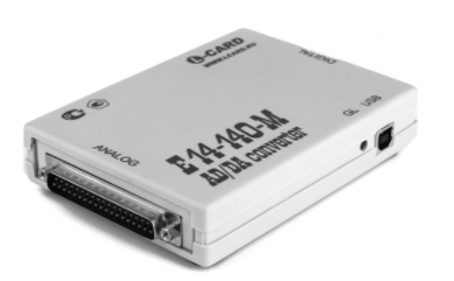
\includegraphics[width=10cm]{images/adc1}
\caption{АЦП LCard E14-140M}
\end{figure}

При работе с данным АЦП возникли трудности при написании програмного обеспечения. Средства разработки ПО для данного ацп давно не обновлялись. Работа с АЦП плохо документирована производителем и приведено мало примеров использования. Тем не менее, удалось запустить данный АЦП на одном из примеров производителя. Данный пример позволяет записывать данные с АЦП в бинарный файл.

\subsubsection{ЛА-н10-12USB}

\begin{table}[H]
\centering
\caption{Технические характеристики АЦП ЛА-н10-12USB}

\begin{tabular}{|l|l|}
                                                                      \hline
Число аналоговых входов            & 2                             \\ \hline
Минимальная частота дискретизации  & 1.25МГц                       \\ \hline
Максимальная частота дискретизации & 80МГц                         \\ \hline
Объем буффера памяти               & $2\times10^{19}=524288$       \\ \hline
Разрядность                        & 12бит (4096 значений)         \\ \hline
Входное сопротивление              & 50Ом                          \\ \hline
Разъем                             & BNC                           \\ \hline
Диапазоны входного напряжения      & $\pm2V;\pm1V;\pm0.4V;\pm0.2V$ \\ \hline
Защита по входному напряжению      & $\pm5V$                       \\ \hline
Дифференциальная нелинейность      & $\pm1.2$ МЗР                  \\ \hline
Интегральная нелинейность          & $\pm1.5$ МЗР                  \\ \hline
Ошибка сдвига                      & $\pm0.15\%$                   \\ \hline
Интерфейс                          & USB                           \\ \hline
Потребляемая мощность              & 12В, 0.7А                     \\ \hline
Масса                              & 400г                          \\ \hline
\end{tabular}
\end{table}

\begin{figure}[H]
\centering
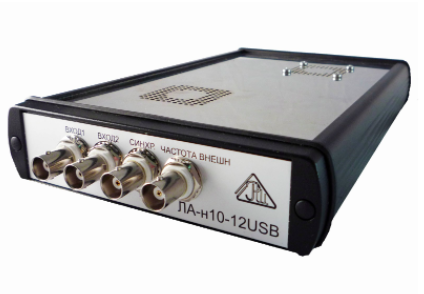
\includegraphics[width=10cm]{images/adc2}
\caption{АЦП ЛА-н10-12USB}
\end{figure}

\textbf{Интегральная нелинейность} - это отклонение точек по вертикальной оси реальной хар-ки от идеальной хар. преобразования, которое делит пополам расстояние по оси X между средними значениями пороговых значений характеристики преобразования. Измеряется в процентах или  МЗР.

\textbf{Дифференциальная нелинейность} - отклонение разности двух аналоговых сигналов от значения, соответствующего единице МЗР.

Для данного АЦП было написано програмное обеспечение, позволяющее принимать данные с АЦП и визуализировать их в реальном времени.

Особенности реализации програмно-аппаратных решений данного АЦП, не позволяющие его использовать в нашем проекте:

Данный АЦП работает в режиме старт-стоп. Другими словами он периодически производит запуск, сбор данных(в буффер) и остановку. Это один полный цикл сбора данных. При этом полезное время - это сбор данных, а старт и стоп - бесполезное.

Время, за которое АЦП совершает полный цикл сбора данных и соотношение полезного и бесполезного времени отличается в зависимости от частоты дискретизации и размера буффера. Были произведены замеры времени для различных значений частоты дискретизации и размера буффера и были составлены следующие таблицы.

Во всех таблицах ось X: размер буффера, ось Y: частота дискр.

\begin{figure}[H]
\centering
% \includegraphics[width=14cm]{sprint-layout-circuit.png}
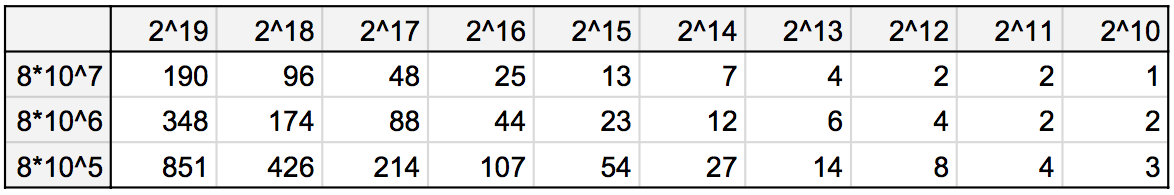
\includegraphics[width=\textwidth]{images/cycle-time.png}
\caption{Время на полный цикл (мс)}
\end{figure}

\begin{figure}[H]
\centering
% \includegraphics[width=14cm]{sprint-layout-circuit.png}
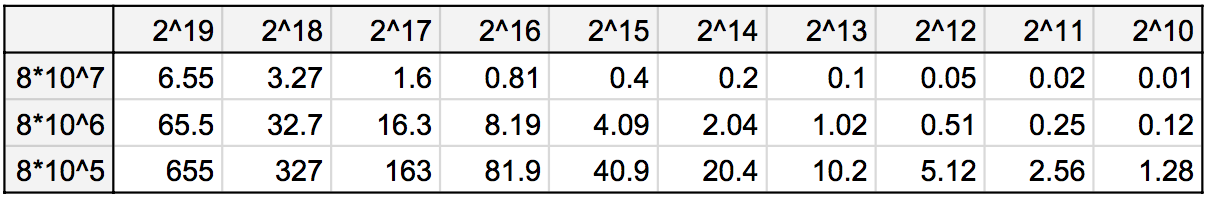
\includegraphics[width=\textwidth]{images/good-time.png}
\caption{Полезное время (мс)}
\end{figure}

\begin{figure}[H]
\centering
% \includegraphics[width=14cm]{sprint-layout-circuit.png}
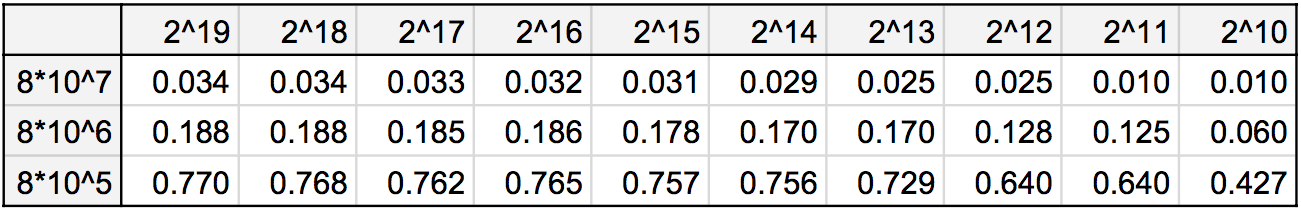
\includegraphics[width=\textwidth]{images/bad-div-by-good.png}
\caption{Отношение полезного времени к полному}
\end{figure}

Как видно из таблицы, даже при самых оптимальных значениях размера буффера и частоты дискретизации, отношение полезного времени к полному составляет 77\%. (полезное время 655мс, полное -  851мс) Тоесть в конце каждого цикла образуется дырка длиной 196мс. При таком долгом времени на перезапуск теряется очень много информации, что неприемлимо для данного проекта. Поэтому было принято решение заменить его. Данный же подходит для коротких сигналов (меньше секунды), которые нужно оцифровывать в сверхвысоком качестве.

\subsubsection{Arduino Due}

Самым оптимальным вариантом АЦП для данного проекта оказался Arduino Due. Он сочетает в себе как простоту в использовании так и возможность оцифровывать сигнал высокого качества. Максимальная частота дискретизации Arduino Due составляет 1МГЦ. В ходе данной работы удалось достичь максимума в 672кГц. Обычно среднее значение частоты дискретизации составляло 666кГц. Максимальное значение частоты дискретизации зависит также от производительности компьютера. Данное устройство тестировалось на MacBook Air 2014.

\begin{figure}[H]
\centering
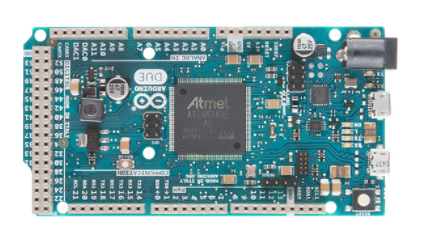
\includegraphics[width=10cm]{images/adc3}
\caption{Технические характеристики АЦП Arduino Due}
\end{figure}

\begin{table}[H]
\centering
\caption{Технические характеристики АЦП Arduino Due}

\begin{tabular}{|l|l|}
                                                                      \hline
Число аналоговых входов            & 12                            \\ \hline
Максимальная частота дискретизации & 1МГц                          \\ \hline
Объем буффера памяти               & 512 KB					               \\ \hline
Разрядность                        & 12бит (4096 значений)         \\ \hline
Рабочее напряжение                 & 3.3V                          \\ \hline
Диапазоны входного напряжения      & 7-12V                         \\ \hline
Защита по входному напряжению      & 6-16V                         \\ \hline
Интерфейс                          & USB                           \\ \hline
Микроконтроллер                    & AT91SAM3X8E                   \\ \hline
Масса                              & 36г                           \\ \hline
\end{tabular}
\end{table}


\end{document}
